\documentclass[10pt]{article}

\usepackage[T1]{fontenc} 
\usepackage[brazilian]{babel} 
\usepackage[utf8]{inputenc} 
\usepackage{algorithm} 
\usepackage{algpseudocode}
\usepackage{amsfonts}
\usepackage{amsmath} 
\usepackage{amssymb}
\usepackage{graphicx,url,float}
\usepackage{latexsym}
\usepackage{sbc-template}
\usepackage{listings} 
\usepackage{color} 
\usepackage{verbatim} 

\lstset{frame=tb,
    aboveskip=3mm,
    belowskip=3mm,
    showstringspaces=false,
    columns=flexible,
    basicstyle={\small\ttfamily},
    numbers=none,
    numberstyle=\tiny\color{gray},
    keywordstyle=\color{blue},
    commentstyle=\color{dkgreen},
    stringstyle=\color{mauve},
    breaklines=true,
    language=python,
    breakatwhitespace=true
    tabsize=3
}

\graphicspath{{images/}}


\sloppy

\title{Programação em Linguagem de Montagem}

\author{Diego Pinto da Jornada}

\address{Faculdade de Informática -- Pontifícia Universidade Católica do Rio Grande do Sul\\
  (PUCRS)
  \email{diego.jornada@acad.pucrs.br}
}

\begin{document} 

\maketitle

\begin{resumo}
    

    
\end{resumo}

\section{Introdução}
\label{sec:intro}

No escopo de disciplina de Organização e Arquitetura de Computadores I o
terceiro trabalho pode ser resumido da seguinte maneira: dado quatro problemas,
estes devem ser resolvidos em uma linguagem de alto nível, no caso deste
trabalho foi escolhido python, e também deve ser apresetnada a solução
utilizando a linguagem assembly do processador cleópatra, como estudado em aula.

Os problemas a serem resolvidos são os seguintes:

\begin{itemize}

    \item Descobrir se um número \emph{n} positivo é múltiplo de número do grupo
        +5(se por acaso, o valor de grupo + 5 ultrapassar o número do maior
        grupo, deve ser subtraído o número do maior grupo.

    \item Fazer um programa que gere os \emph{n} primeiros números da sequência
        de Fibonnacci, e armazene a sequências em endereços consecutivos a
        partir da posição de memória com rótulo idx. Esta operação deve ser
        feita com uma chamada de função para o rótulo SeqFibonnacc i.  

    \item Faça um programa que calcule a multiplicação de todos os elementos da
        diagonal principal de uma matriz 5x5. Obs.: o algoritmo deve ser
        genérico para qualquer matriz quadrada. Este programa deve chamar
        uma função para fazer a multiplicação


    \item Faça um programa que contenha a função Potencia. Esta função deve
        ser capaz de receber dois valores \emph{V} e \emph{EXP} e ter como
        saída $V{exp}$. Esta saída deve estar associada ao acumulador


\end{itemize}


\section{Exercício 1}

O exercício um é o seguinte: Descobrir se um número \emph{n} positivo é múltiplo
de número do grupo +5(se por acaso, o valor de grupo + 5 ultrapassar o número do
maior grupo, deve ser subtraído o número do maior grupo.

O o grupo deste trabalho é o grupo 1, logo o exercicío será ver se um número é
divisível por 6.

\subsection{Descrição Alto Nível}

A desrição em alto nível foi utilizando a linguagem python é desta forma:

\begin{lstlisting}

def div(n, grupo):
    divisor = grupo + 5
    res = n
    while res >= grupo:
        res -= divisor
    
    return res

\end{lstlisting}

\subsection{Descrição Baixo nível}
\begin{verbatim}
    
.CODE
    lda grupo
    add #5
    not
    add #1
    sta divisor
    lda num
    sta resto
    ENQUANTO:
        lda resto
        add divisor
        jz  DIVIDE 
        jn  SOBRA
        sta resto
        jmp ENQUANTO
    SOBRA:
        lda #0
        sta resp
        jmp FIM
    DIVIDE:
        lda #1
        sta resp        
    FIM:
        hlt
.ENDCODE

.DATA
   num:     db  #12 ;Num a ser testado 
   resp:    db  #01
   grupo:   db  #1
   divisor: db  #0
   resto:   db  #0
.ENDDATA
\end{verbatim}

\subsection{Tela Montador}

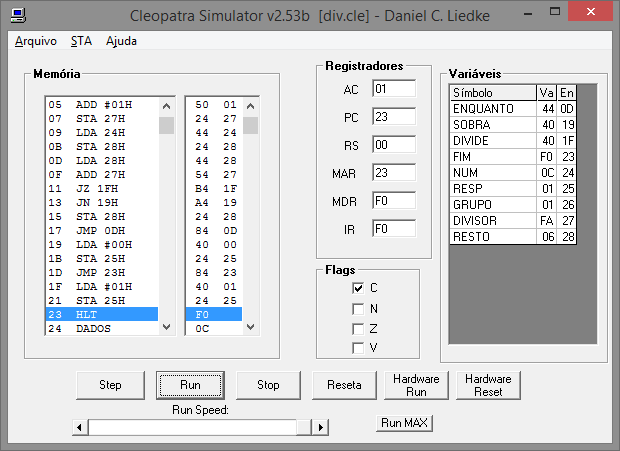
\includegraphics{images/div.png}

\subsection{Contagem Operações e estimativa de de tempo de execução}

Considerando \emph{num} como \emph{x} temos a seguinte função:
$$f(x) = 40x + 88$$

O Tempo de excução seria 0.000568ms para x=12 ao considerarmos que o Cleópatra
opera a 1GHz.


\section{Exercício 7}

    Faça um programa que contenha a função Potencia. Esta função deve ser capaz
    de receber dois valores \emph{V} e \emph{EXP} e ter como saída $V{exp}$.
    Esta saída deve estar associada ao acumulador

\subsection{Descrição Alto Nível}

A desrição em alto nível foi utilizando a linguagem python é desta forma:

\begin{lstlisting}

def pot(n, exp):
    res = 1
    while exp > 0:
        res = mult_sum(res, n)        
        exp -=1
    return res


def mult_sum(a, b):
    res = 0
    while b > 0:
        res += a
        b-=1
    return res

\end{lstlisting}
Note que foi usada uma função auxiliar para fazer a multiplicação atraveś de
soma isso para que a descrição em alto nível seja mais parecida com a
implementação de baixo nível. 

\subsection{Descrição Baixo nível}
\begin{verbatim}
    
.CODE
INIT:
	lda exp
	jz  FIM,R
	jsr MULT_SUM,R
	sta res
	lda exp
	add #-1
    sta exp
	jmp INIT
		MULT_SUM:
            lda #0
            sta resAux
		lda n
		sta aux
		LOOP2:
			jz FIMLOOP2,R
			add #-1
			sta aux
			lda resAux
			add res
			sta resAux
			lda aux
			jmp LOOP2,R
		FIMLOOP2:
			lda resAux
			rts
	FIM:
		hlt
.ENDCODE

.DATA
	n:		db	#3
	exp:		db	#3
	res:	db	#1      ;respota

	aux:	db	#0      
	resAux:	db	#0
.ENDDATA

\end{verbatim}

\subsection{Tela Montador}

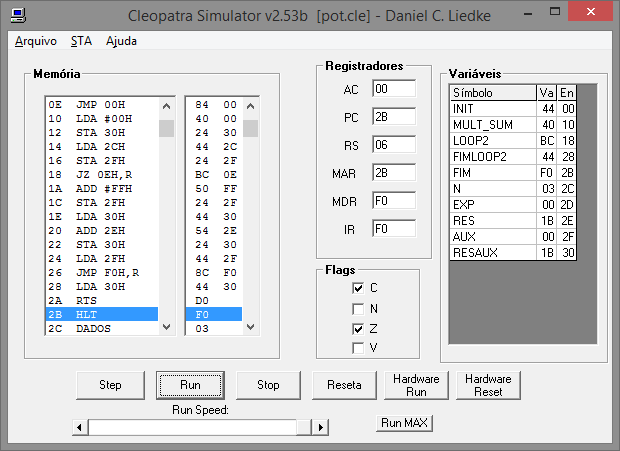
\includegraphics{images/pot.png}

\subsection{Contagem Operações e estimativa de de tempo de execução}

Considerando \emph{n} como \emph{x} e \emph{exp} como \emph{y} temos a seguinte função:
$$73y + 46xy + 39$$
O Tempo de excução seria 0.000672ms para x e y valendo 3, ao considerarmos que o Cleópatra opera a
1GHz.


\section{Exercício 12}

    Fazer um programa que gere os \emph{n} primeiros números da sequência de
    Fibonnacci, e armazene a sequências em endereços consecutivos a partir da
    posição de memória com rótulo idx. Esta operação deve ser feita com uma
    chamada de função para o rótulo SeqFibonnacci.  

\subsection{Descrição Alto Nível}

A desrição em alto nível foi utilizando a linguagem python é desta forma:

\begin{lstlisting}

def fib(n):
    a, b, c = 0, 1, 0
    res = []
    while c < n:
        res[a] = b
        a, b = b, a+b
        c+=1

\end{lstlisting}

\subsection{Descrição Baixo nível}
\begin{verbatim}
    
.CODE
INIT:	
	lda #0
	sta n1
	lda #1
	sta n2
	lda p
	add #2
	sta p
	lda n
	add #-2
	sta n
	LOOP:
		jz	FIM
		jsr SEQFIBONACCI
		lda	p
		add	#1
		sta p
		lda n
		add	#-1
		sta	n
		jmp LOOP
			SEQFIBONACCI:
				lda n1
				add n2
				sta nxt
				sta p,I
				lda n2
				sta n1
				lda nxt
				sta n2
				rts     
FIM:
	hlt
                     
.ENDCODE

.DATA
    n:      db  #10      ;Seq FIB
    n1:     db  #0		 ;fib-2
    n2:     db  #0		 ;fib-1
    nxt:    db  #0		 ;n1 + n2
    p:      db  #idx
    idx:    db  #0, #1, #0, #0, #0, #0, #0
.ENDDATA

\end{verbatim}

\subsection{Tela Montador}

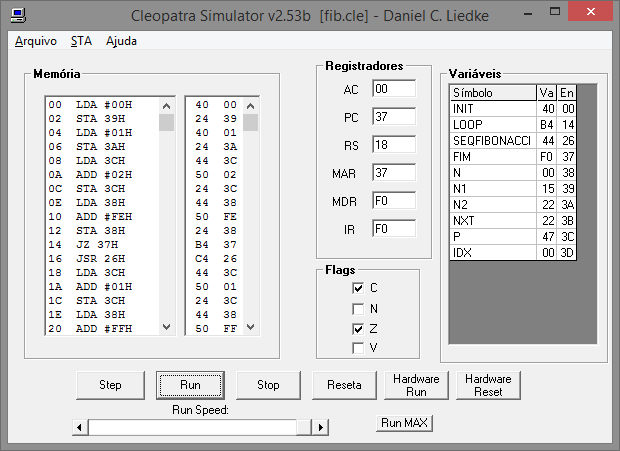
\includegraphics{images/fib.png}

\subsection{Contagem Operações e estimativa de de tempo de execução}

Considerando \emph{n} como \emph{x} temos a seguinte função:
$$f(x) = 124x + 65$$
O Tempo de excução seria xxx ao considerarmos que o Cleópatra opera a
1GHz.



\section{Exercício 21}

 Faça um programa que calcule a multiplicação de todos os elementos da diagonal
 principal de uma matriz 5x5. Obs.: o algoritmo deve ser genérico para qualquer
 matriz quadrada. Este programa deve chamar uma função para fazer a
 multiplicação

\subsection{Descrição Alto Nível}

A desrição em alto nível foi utilizando a linguagem python é desta forma:

\begin{lstlisting}

def diag(matrix):
    res = 1
    for i in range(len(matrix)):
        el = matrix[i][i]
        res = mult_sum(res, el)
    return res


def mult_sum(a, b):
    res = 0
    while b > 0:
        res += a
        b-=1
    return res

\end{lstlisting}

\subsection{Descrição Baixo nível}
\begin{verbatim}
    
.CODE
	lda	size
	JZ	FIM
	sta	aux
	lda	aux
INIT:
	jz	FIM,R
	lda	m
	add	mov
	sta	value
	jsr	MULT_SUM,R
	lda	mov
	add	#1
	add	size
	sta	mov
	lda	aux
	add	#-1
	sta	aux
	JMP	INIT,r
		MULT_SUM:
			lda	#0
			sta	multAux
			lda	value,I
			sta	val
			LOOP:
				jz	RETURN,R
				add	#-1
				sta	value
				lda	multAux	
				add	res
				sta	multAux
				lda	value
				jmp	LOOP,R
			RETURN:
				lda multAux
				sta res
				rts
FIM:
	hlt
.ENDCODE

.DATA

	res:	db	#1
	size:	db	#5    	
	m:	db	a, b, c, d, e
	a:	db	#1, #6, #7, #8, #9
	b:	db	#10, #2, #11, #12, #13
	c:	db	#14, #8, #3, #16, #17
	d:	db	#18, #19, #20, #4, #21
	e:	db	#22, #23, #24, #25, #5
	aux:	db	#0
	mov:	db	#0
	value:	db	#0
	multAux:db	#0
	val:	db	#0

.ENDDATA

\end{verbatim}

\subsection{Tela Montador}

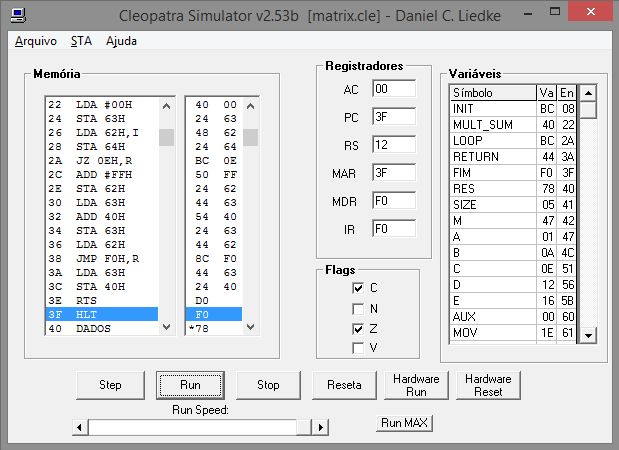
\includegraphics{images/matrix.png}

\subsection{Contagem Operações e estimativa de de tempo de execução}

Considerando \emph{n} como \emph{x} temos a seguinte função:
$$f(x) = 196x + 32$$
O Tempo de excução seria xxx ao considerarmos que o Cleópatra opera a
1GHz.



\bibliographystyle{sbc}
\bibliography{report}

\end{document}
